\documentclass[a4paper,10pt]{article}
\usepackage[utf8]{inputenc}
\usepackage{listings}
\usepackage{graphicx}
\usepackage{subcaption}
\usepackage{adjustbox}
\usepackage{hyperref}
\usepackage{imakeidx}

\title{Compte rendu TP : Architecture logicielle}
\date{29/05/21}
\author{Hamze Al-Rasheed - Nicolas Commandeur - Benjamin Verdant - Robin Wagner}

\begin{document}
    \maketitle
    \pagenumbering{gobble}
    \newpage
    \tableofcontents
    \newpage
    \pagenumbering{arabic}
    
    \section{Sujet}
        Le principe du tp est de concevoir l'architecture d'un système de contrôle d'accès à un ensemble de bâtiments.
    
        Un batiment possède un nom ainsi que des informations. Les informations sont :
        \begin{itemize}
            \item la liste des portes du bâtiment
            \begin{itemize}
                \item Le nom de la porte    \newline
                \textit{ex : Porte sud, 8A-44, etc}
                \item L'id de la badgeuse d'entrée et de sortie de la porte
                \newline
                Impair pour entrer et pair pour sortir \newline
                \textit{ex : 11 pour entrer dans le bâtiment 1 et 12 pour en sortir}
                \item La liste des cartes autorisées ou non 
                \newline
                \textit{ex : Badgeuse 11 : carte 1 autorisée, carte 2 non autorisée, etc}
                \item L'état de la porte
                \newline
                \textit{ex : Ouvert ou fermé}
            \end{itemize}
        \end{itemize}
        
        Les utilisateurs ont chacun une \textbf{carte} qui a un \textbf{id} unique et le nom du détenteur de celle-ci.
        \newline
        \textit{ex : carte 1 $\Rightarrow$ Livai, carte 2 $\Rightarrow$ Eren }

        Pour accéder à un bâtiment ou à une salle, un utilisateur doit poser sa carte sur la badgeuse.
        \newline
        \par Si la personne \underline{est autorisée} à entrer dans le bâtiment alors, la porte s'ouvre et une lumière verte s'affiche pendant \textbf{15 secondes} et la porte reste ouverte pendant le \textbf{même temps}.
        \newline
        Si la personne n'est pas autorisée à entrer dans le bâtiment, une lumière rouge s'allume sur celle-ci.
        \newline
        \par
        Quand une personne ouvre une porte, un laser se situe juste après celle-ci, pour compter le nombre de personne qui passe. Plusieurs cas possibles :
        \begin{itemize}
            \item Une seule personne passe $\Rightarrow$ la personne qui a ouvert la porte est enregistrée dans le bâtiment et une trace de son passage est inscrit dans le log des passages.
            \item Plusieurs personnes passent $\Rightarrow$ une alarme retentit
            \item Personne ne passe $\Rightarrow$ rien ne se passe
        \end{itemize}

        Dans tous les cas, la porte se ferme au bout de \textbf{15 secondes}
        \newline

        \par En cas d'un incendie, toutes les portes sont débloquées et on inscrit dans un fichier toutes les personnes dans les bâtiments.
        \pagebreak
    \section{Prémice}
    Tout d'abord, nous avons analysé le sujet puis nos avons fait un diagramme de classe et un prototype d'un diagramme de séquence. Nous nous en sommes servis de base que nous avons au fur-à-mesure modifier.

    \begin{figure}[h]
        \begin{subfigure}{1.0\textwidth}
            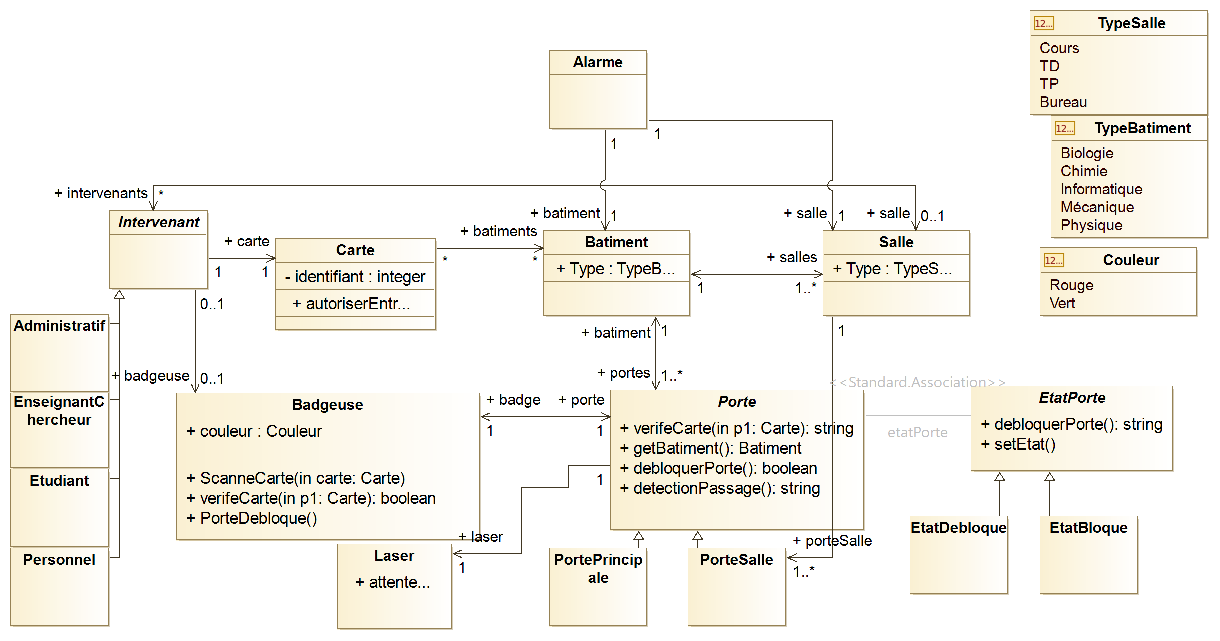
\includegraphics[width=1\linewidth, height=4cm]{image/classe.png}
             \caption{Diagramme de classe}
             \label{fig:classe}
        \end{subfigure}
        \newline
        \newline
        \newline

        \begin{subfigure}{1.0\textwidth}
            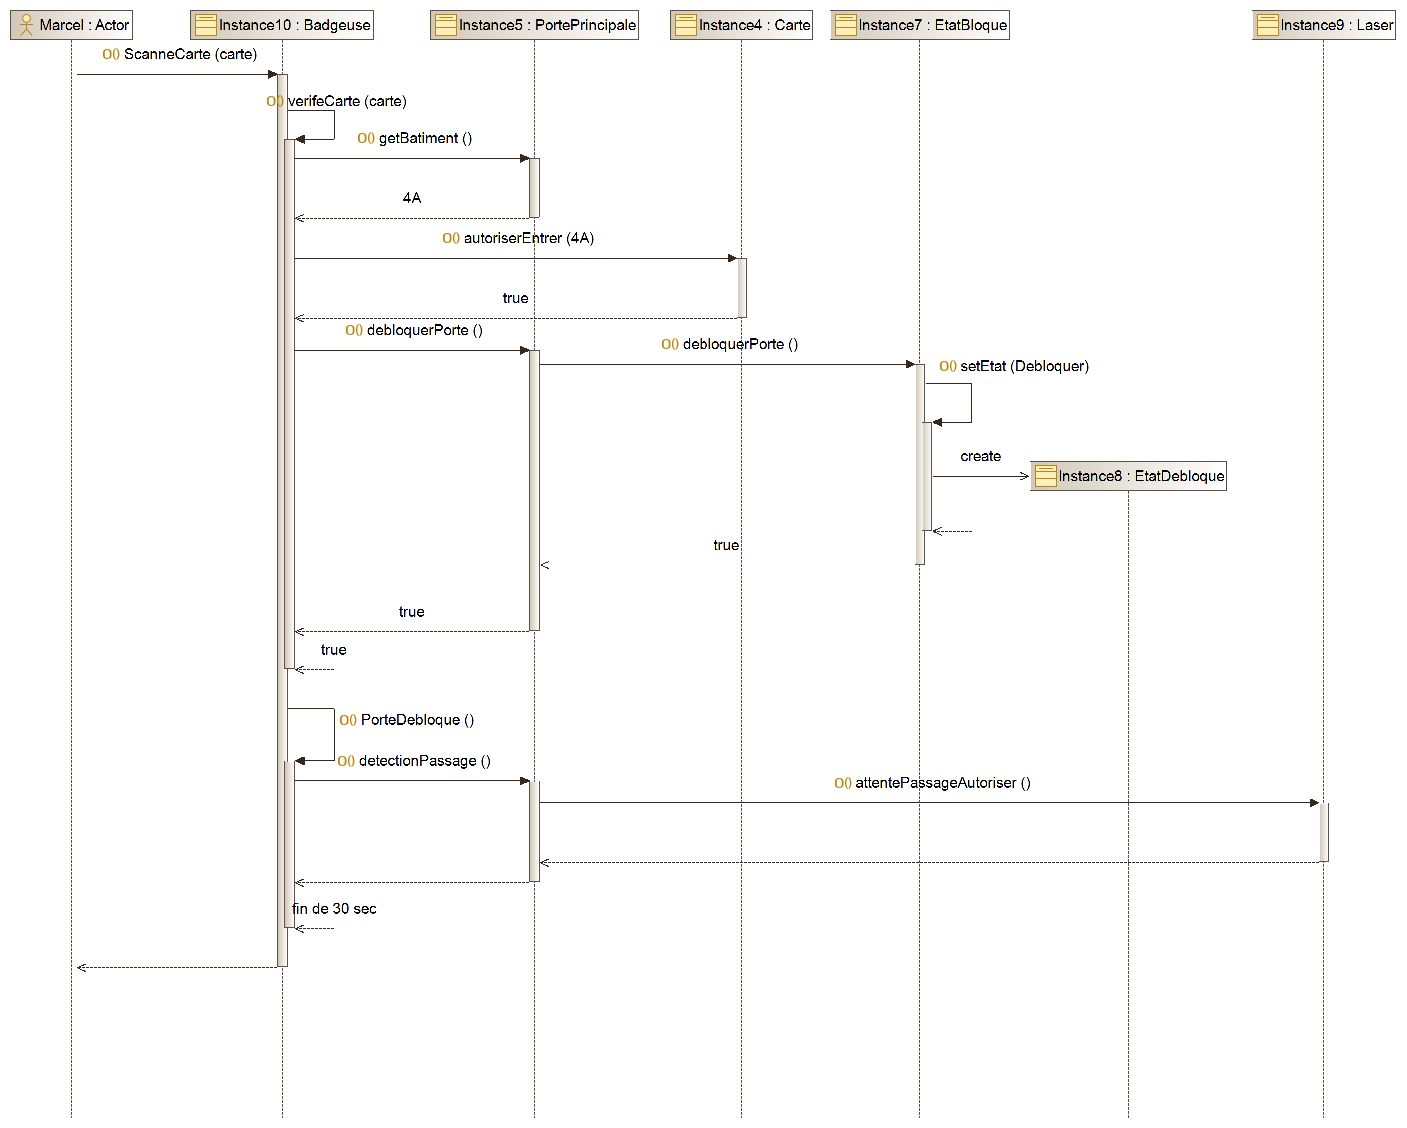
\includegraphics[width=1\linewidth, height=4cm]{image/sequence.png}   
            \caption{Diagramme en séquence}
            \label{fig:sequence}
        \end{subfigure}
    \end{figure}

    \pagebreak
    \section{Architecture utilisée}
    \pagebreak
    \section{Choix technologiques}
    \pagebreak
    \section{Petit pas pour l'homme}
    \pagebreak
    \section{Grand pas pour l'humanité}
    \pagebreak
    \section{Difficultés rencontrées}
    \pagebreak
    
\end{document}